% Created 2016-05-02 mån 18:07
% Intended LaTeX compiler: pdflatex
\documentclass{scrartcl}
\usepackage[utf8]{inputenc}
\usepackage[T1]{fontenc}
\usepackage{graphicx}
\usepackage{grffile}
\usepackage{longtable}
\usepackage{wrapfig}
\usepackage{rotating}
\usepackage[normalem]{ulem}
\usepackage{amsmath}
\usepackage{textcomp}
\usepackage{amssymb}
\usepackage{capt-of}
\usepackage{hyperref}
\usepackage{khpreamble}
\newcommand{\tustin}{\frac{2}{h}\frac{z-1}{z+1}}
\author{Kjartan Halvorsen}
\date{2016-04-29}
\title{Computerized control - final exam (dummy)}
\hypersetup{
 pdfauthor={Kjartan Halvorsen},
 pdftitle={Computerized control - final exam (dummy)},
 pdfkeywords={},
 pdfsubject={},
 pdfcreator={Emacs 24.5.1 (Org mode 8.3.4)}, 
 pdflang={English}}
\begin{document}

\maketitle

\section*{Problem 1}
\label{sec:orgheadline1}
The figure below shows the poles of a continuous-time transfer function representing the dynamics of a system.
\begin{center}
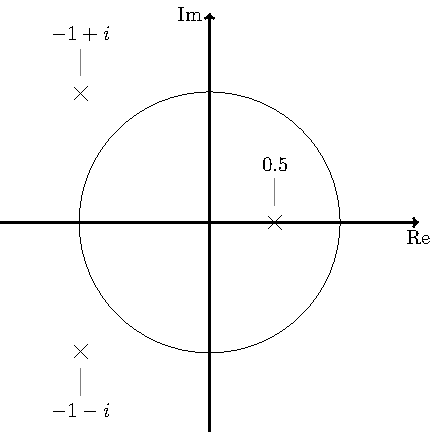
\includegraphics[width=0.3\linewidth]{imaginary-plane-ct-poles}
\end{center}
Choose a reasonable sampling period \(h\), and plot the poles of the discrete-time system obtained by zero-order-hold sampling
\begin{center}
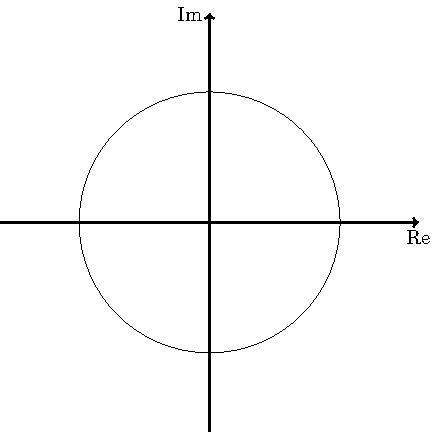
\includegraphics[width=0.3\linewidth]{imaginary-plane-empty}
\end{center}

\section*{Problem 2}
\label{sec:orgheadline5}
Circle the correct answer to each question. Motivate your answer briefly with 1-2 sentences.

\subsection*{(a)}
\label{sec:orgheadline2}
\begin{center}
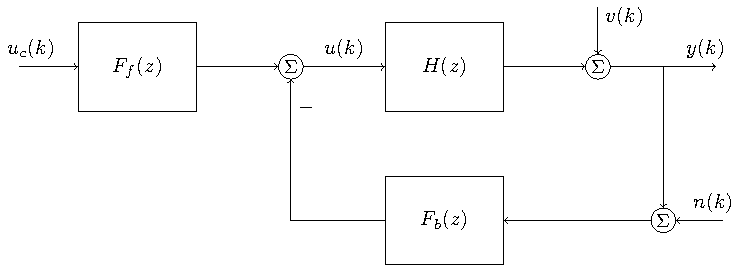
\includegraphics[width=0.6\linewidth]{../../homework/2dof-block-complete}
\end{center}
The figure above shows a block-diagram of two-degrees-of-freedom control system. Which of the following pulse transfer operators describes the \textbf{closed-loop response}, \(y(kh)\), to the measurement noise sequence, \(n(kh)\).    
\begin{enumerate}
\item \(H_n(q) = \frac{1}{1 + G(q)F_b(q)}\)
\item \(H_n(q) = -\frac{G(q)F_f(q)}{1 + G(q)F_f(q)}\)
\item \(H_n(q) = -\frac{G(q)F_b(q)}{1 + G(q)F_b(q)}\)
\item \(H_n(q) = \frac{G(q)F_b(q)}{1 + G(q)F_b(q)}\)
\end{enumerate}

\subsection*{(b)}
\label{sec:orgheadline3}
The continuous-time harmonic oscillator has transfer function
\[ G(s) = \frac{\omega^2}{s^2 + \omega^2}. \]
Zero-order hold sampling of the system gives the pulse transfer function
\begin{enumerate}
\item \(H(z) = \frac{(1-\cos\omega h)(z+1)}{(z-\cos \omega h)^2 + \sin^2 \omega h}\)
\item \(H(z) = \frac{(1-\cos\omega h)(z+1)}{(z-1)^2 + \sin^2 \omega h}\)
\item \(H(z) = \frac{(1-\cos\omega h)(z+1)}{(z+\cos \omega h)^2 + \sin^2 \omega h}\)
\end{enumerate}

\subsection*{(c)}
\label{sec:orgheadline4}
The figure below shows the step-response of a closed-loop system with a discretized PID controller for some values of the controller parameters. In continuous-time the controller has the form
 \[ F(s) = K\Big(1 + \frac{1}{T_i s} + \frac{T_ds}{1 + T_ds/N}\Big). \]
\begin{center}
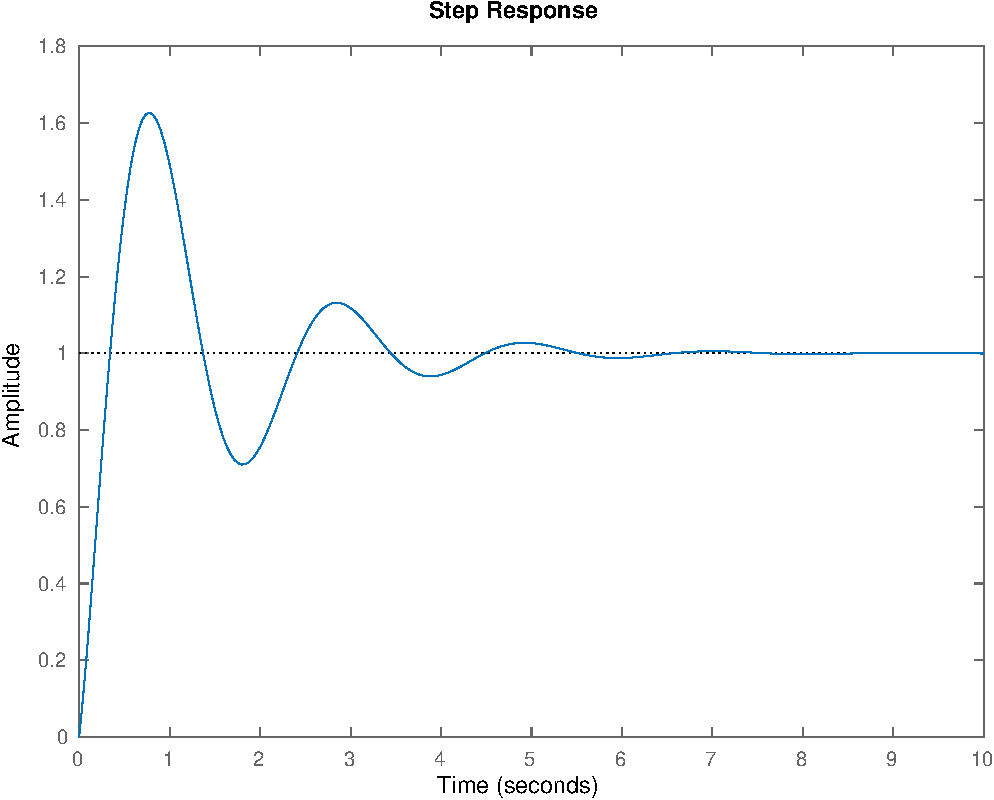
\includegraphics[width=0.4\linewidth]{tuned-response}
\end{center}
How should the controller be modified if we want the response of the closed-loop system to be \textbf{faster with less overshoot}?
\begin{enumerate}
\item Increase \(N\) and decrease \(T_i\).
\item Increase \(K\) and \(T_d\).
\item Decrease \(K\) and increase \(T_d\).
\item Increase \(K\) and decrease \(T_i\).
\end{enumerate}


\section*{Problem 3}
\label{sec:orgheadline8}
Consider the discrete-time double integrator
\[ H(z) = \frac{h^2(z+1)}{2(z-1)^2}. \]
\subsection*{(a)}
\label{sec:orgheadline6}
Write the system on state-space form, using the controllable canonical form
\begin{equation*}
  \begin{split}
  x(k+1) &= \underbrace{\bbm -a_1 & -a_2 & \cdots & - a_{n-1} & -a_n\\
                  1  &   0   &  \cdots & 0        &   0\\
                  0  &   1   &  \cdots & 0        &   0\\
                  \vdots &\vdots & \ddots & \vdots&   \vdots\\
                  0  &   0   &  \cdots & 1        &   0
             \ebm}_{\Phi}
	     x(k) + \underbrace{\bbm 1\\0\\0\\\vdots\0\ebm}_{\Gamma} u(k), \\
  y(k) &= \bbm b_1 & b_2 & \cdots & b_n \ebm x(k)
  \end{split}
 \end{equation*}
where
\[ H(z) = \frac{b_1z^{n-1} + b_2z^{n-2} + \cdots + b_n}{z^n + a_1z^{n-1} + \cdots + a_n}. \]

\subsection*{(b)}
\label{sec:orgheadline7}
Determine a linear state feedback
\[ u(k) = -Lx(k) + u_c(k) \]
such that the closed-loop system has poles in \(\pm i0.4\)

\section*{Solutions}
\label{sec:orgheadline17}
\subsection*{Problem 1}
\label{sec:orgheadline9}
The system has two stable, complex-conjugated poles with distance \(\omega_0 = \sqrt{2}\) from the origin, and one unstable pole in \(s=0.5\). The two stable poles are faster than the unstable pole, since they are farther from the origin. We can use the rule-of-thumb
\[ \omega_0 h \approx 0.2 - 0.6, \]
but we should be cautious and choose a sampling period in the shorter end of the range. The reason is that zero-order-hold implies a time-delay of approximately \(h/2\), and time-delays in unstable systems are problematic.

With \(\omega_0h=0.2\) we get the discrete time poles
\begin{center}
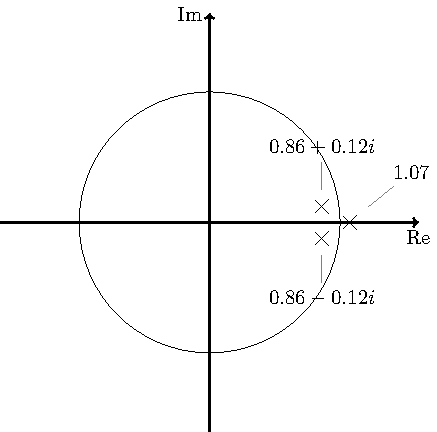
\includegraphics[width=0.3\linewidth]{imaginary-plane-dt-poles}
\end{center}

\subsection*{Problem 2}
\label{sec:orgheadline13}

\subsubsection*{(a)}
\label{sec:orgheadline10}
The correct answer is: 3. \(H_n(q) = -\frac{G(q)F_b(q)}{1 + G(q)F_b(q)}\). We can calculate the transfer function to find this answer, or argue as follows. There is a minus sign (negation) in the path from \(n\) to \(y\), so the pulse transfer operator must be negative. Only alternatives 2 and 3 are negative. Of these two, alternative 2 includes the pulse transfer operator \(F_f(q)\), but \(F_f(q)\) is outside the signal path from \(n\) to \(y\).

\subsubsection*{(b)}
\label{sec:orgheadline11}
The correct answer is: 1. \(H(z) = \frac{(1-\cos\omega h)(z+1)}{(z-\cos \omega h)^2 + \sin^2 \omega h}.\)
The harmonic oscillator has poles on the imaginary axis in the continuous-time case, and on the unit circle in the discrete-time case. Both alternative 1 and 3 have poles on the unit circle. However, the discrete-time poles are obtained from the continuous-time poles \(\pm i\omega\) according to the mapping
\[ p = \mexp{\pm i\omega h} = \cos\omega h \pm i\sin\omega h, \]
where the last equality is the famous Euler's formula. Alternative 1 has indeed poles in 
\[ \cos\omega h \pm i \sin\omega h, \]
whereas Alternative 3 has poles in 
\[ -\cos\omega h \pm i \sin\omega h. \]

\subsubsection*{(c)}
\label{sec:orgheadline12}
The correct answer is:  2. Increase \(K\) and \(T_d\). To make the response faster, we must increase the gain of the controller \(K\). Only alternative 2 and 4 suggest this. To make the overshoot smaller, we must increase the damping. This is done by increasing \(T_d\). 

\subsection*{Problem 3}
\label{sec:orgheadline16}

\subsubsection*{(a)}
\label{sec:orgheadline14}
The harmonic oscillator can be written
\[ H(z) = \frac{h^2(z+1)}{2(z-1)^2} = \frac{h^2/2(z+1)}{z^2-2z + 1}, \]
which  on controllable canonical form is 
   \begin{equation*}
 \begin{split}
  x(k+1) &= \bbm 2 & -1\\1 & 0 \ebm x(k) + \bbm 1\\0\ebm u(k)\\
  y(k) &= \bbm h^2/2 & h^2/2 \ebm .
 \end{split}
\end{equation*}

\subsubsection*{(b)}
\label{sec:orgheadline15}
Linear feedback control of a system on controllable canonical form is particularly easy, since the resulting system is also on controllable canonical form. The closed loop system with
\[ u(k) = -Lx(k) + u_c(k) \]
has pulse transfer function
\[ H_c(z) = \frac{h^2/2(z+1)}{z^2 (-2+l_1)z + 1+l_2} \]
and the desired denominator is
\[ (z-i0.4)(z+i0.4) = z^2 + 0.4^2, \]
Equating the coefficients gives the feedback gains
\begin{align*}
-2+l_1 &= 0 \quad \Rightarrow \quad l_1 = 2\\
1+l_2 &= 0.16 \quad \Rightarrow \quad l_2 = -0.84
\end{align*}

A step-response with \(h=1\) and a step in \(u_c\) occurring at \(t=1\) is shown below.
\begin{center}
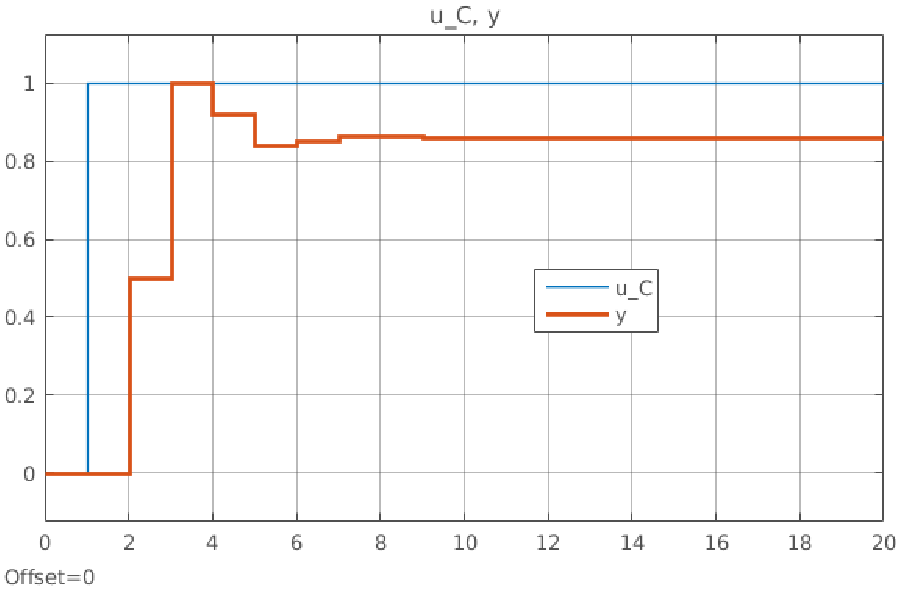
\includegraphics[width=0.6\linewidth]{problem3_dummy_step_response-crop}
\end{center}
\end{document}